Overview of this part.

\chapter{Memory Object Models, explained}\label{chap:mem-model-explained}

Explain the connection to Core \textemdash{} not that strong, thanks to the memory
interface and the invariants of the VIP heaps, separation logic heaps, and
memory actions.

Factorising the formalisation pays off here.

\chapter{Pointers: more than you wanted to know}

Explain pointers in excrutiating detail, and why we need provenance for
optimisations.

Why do we care about provenance, why are pointers not just addresses

Common-subexpression elimination, copy-propogation, etc.

\section{Explaining PNVI-ae-udi and VIP}

Why you need provenance.

\section{Design Space}

Alternatives

\begin{figure}[h]
    \centering
    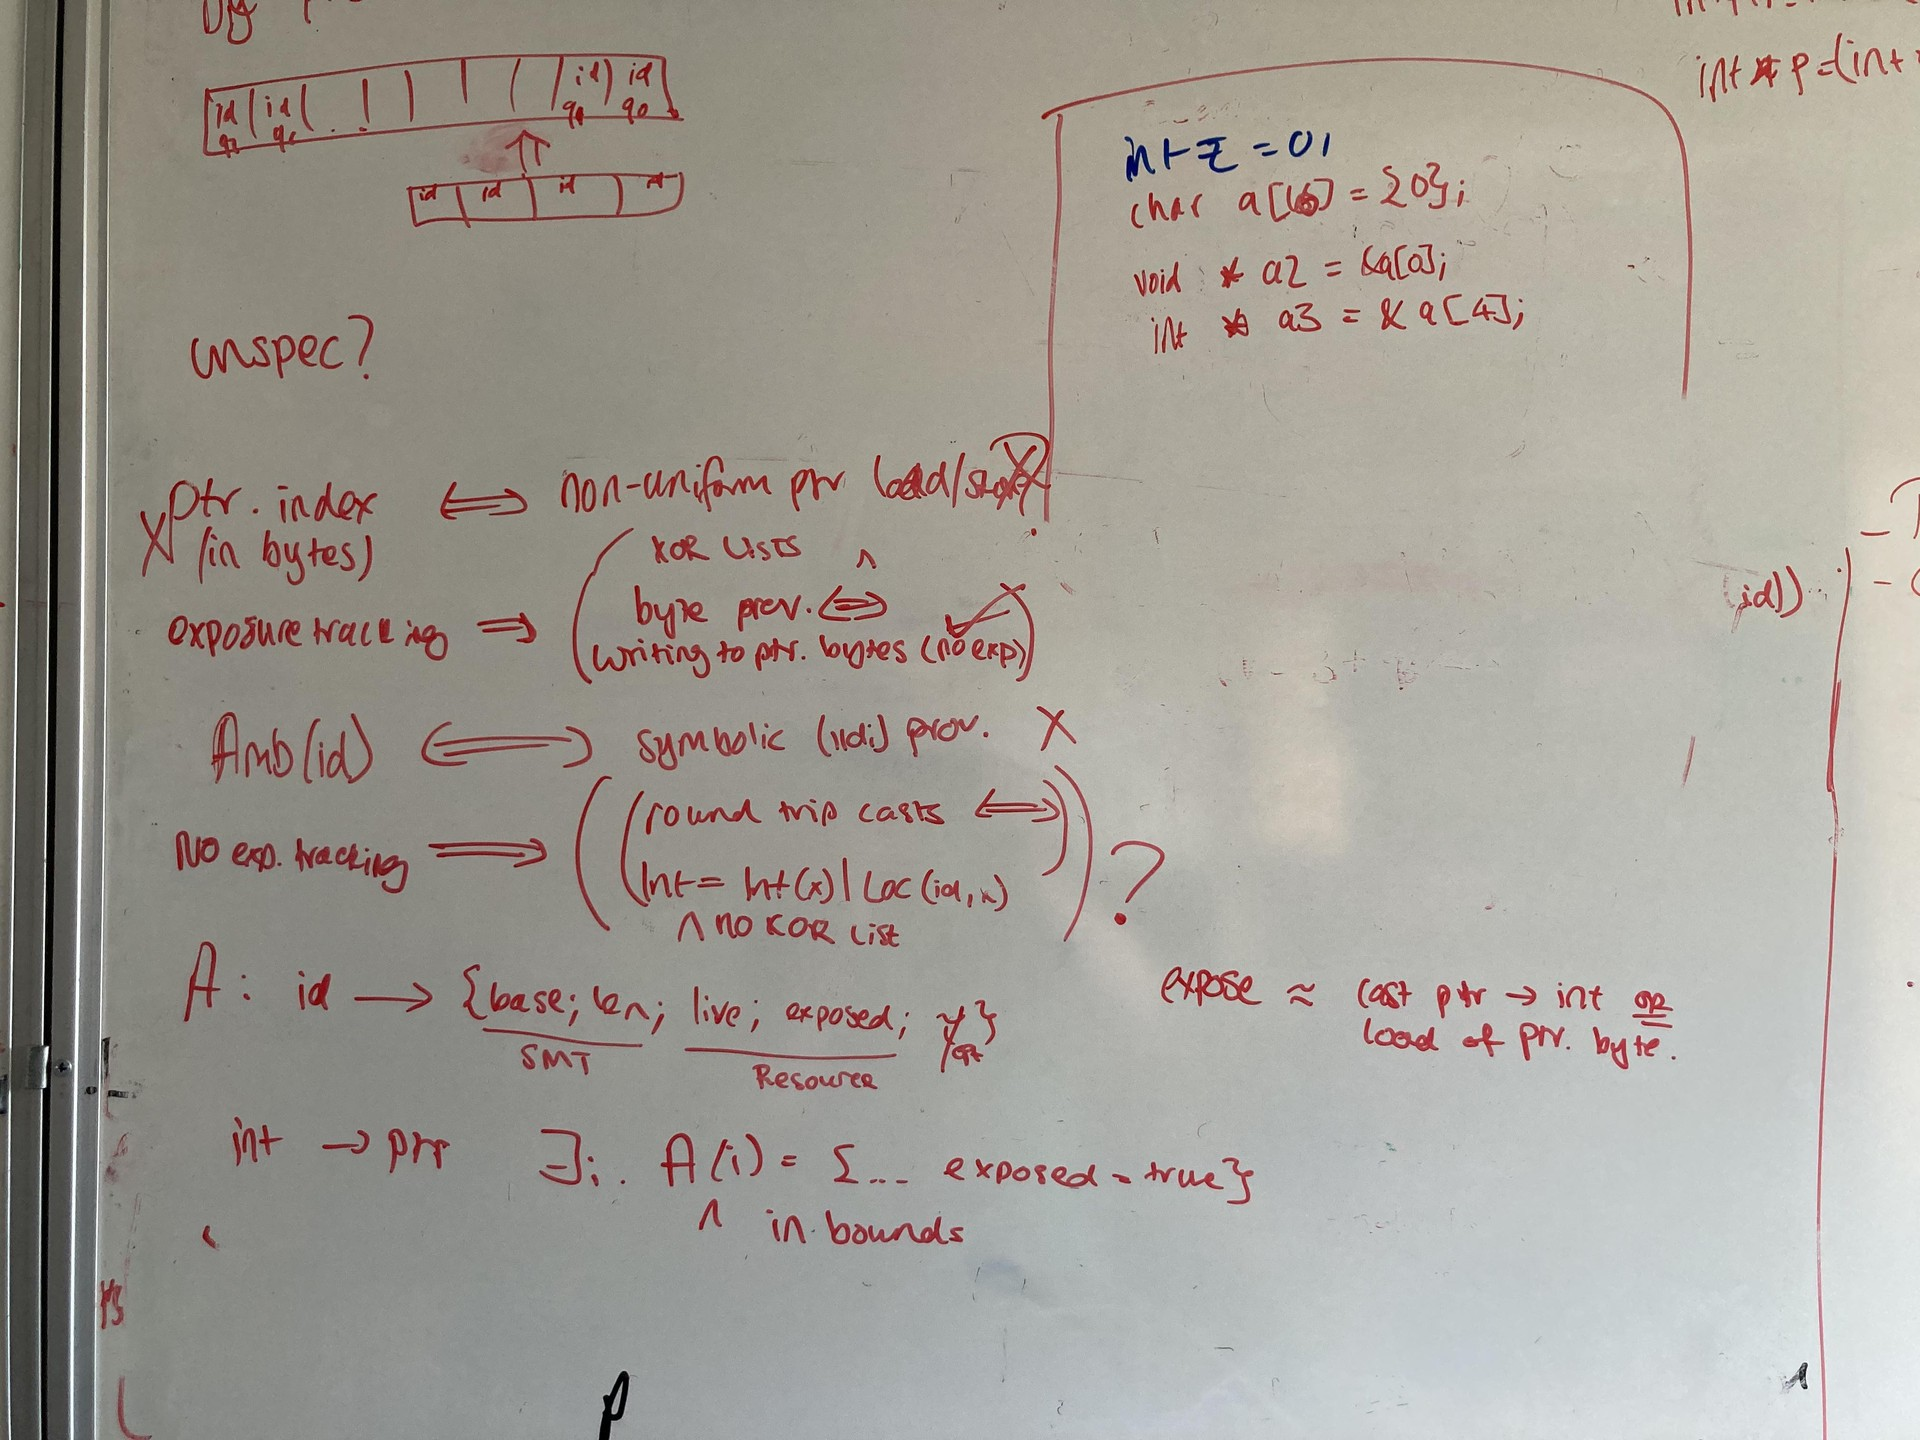
\includegraphics[width=\textwidth]{../misc/type-system-options.jpg}
\end{figure}


\section{Implementation}

Performance graph

\begin{figure}[h]
    \centering
    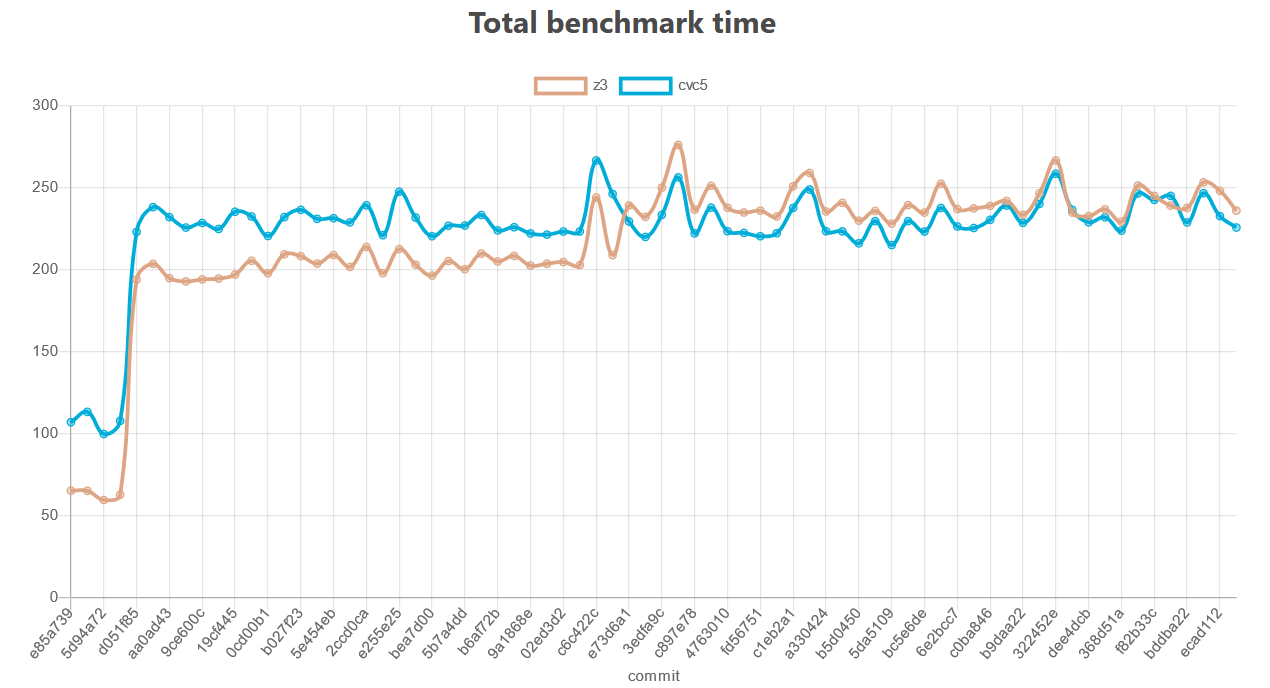
\includegraphics[width=\textwidth]{../misc/vip-performance-hit.png}
\end{figure}

\url{https://rems-project.githb.io/cerberus/dev/bench/}

